\documentclass[a4paper,12pt]{article}
\usepackage{polski}
\usepackage[utf8]{inputenc}
\usepackage[left = 3cm, right = 3cm, top = 2cm, bottom = 2cm]{geometry}
\usepackage{enumerate}
\usepackage{amssymb}		% pakiet do symboli
\usepackage{mathtools}		% pakiet do matmy (rozszerza amsmath)
\usepackage{enumitem}		% punktowanie (a), (b), ...
\usepackage{nopageno}		% brak numerow stron
\usepackage{graphicx}		% wstawianie obrazkow
\usepackage{float}			% wstawianie obrazkow w dowolnym miejscu
\usepackage{caption}
\usepackage{esdiff}         % pochodne \diff{}{}
\usepackage{listings}
\usepackage{xcolor}
\usepackage{adjustbox}
\usepackage{tkz-graph}
%\usepackage[none]{hyphenat} % usunięcie łamania wyrazów na końcu linii

% nowe komendy dla wygodniejszego pisania :)

\newcommand{\floor}[1]{\left\lfloor #1 \right\rfloor}	% podłoga
\newcommand{\ceil}[1]{\left\lceil #1 \right\rceil}		% sufit
\newcommand{\fractional}[1]{\left\{ #1 \right\}}		% część ułamkowa {x}
\newcommand{\abs}[1]{\left| #1 \right|}					% wartosc bezwzgledna / moc
\newcommand{\set}[1]{\left \{ #1 \right \}}				% zbiór elementów {a,b,c}
\newcommand{\pair}[1]{\left( #1 \right)}				% para elementów (a,b)
\newcommand{\Mod}[1]{\ \mathrm{mod\ #1}}				% lekko zmodyfikowane modulo
\newcommand{\comp}[1]{\overline{ #1 }} 					% dopełnienie zbioru 
\newcommand{\annihilator}{\mathbf{E}}					% operator E
\newcommand{\seqAnnihilator}[1]{\annihilator \left\langle #1 \right\rangle} % E(a_n)
\newcommand{\sequence}[1]{\left\langle #1 \right\rangle} % <a_n>
\DeclareMathOperator{\lcm}{lcm}							% obsługa lcm w mathmode

% styl do kodu
\lstdefinestyle{code}{%
basicstyle=\ttfamily\small,
commentstyle=\color{green!60!black},
keywordstyle=\color{magenta},
stringstyle=\color{blue!50!red},
showstringspaces=false,
numbers=left,
numberstyle=\footnotesize\color{gray},
numbersep=10pt,
tabsize=4,
rulecolor=\color{red},
breaklines=true
}

\newcommand{\code}[1]{\lstinline[style=code]{#1}} % kod inline

\begin{document}
\noindent \textbf{Matematyka dyskretna L, Lista 11 - Tomasz Woszczyński}\newline

\noindent \newline \textbf{Zadanie 1 (-)} \newline
Udowodnij lub obal: Nie istnieje graf eulerowski (tj. zawierający cykl Eulera)
o parzystej liczbie wierzchołków i nieparzystej liczbie krawędzi. \\

\noindent Graf eulerowski to taki, w którym istnieje cykl Eulera, a więc cykl
przechodzący przez wszystkie krawędzie dokładnie raz. Stwierdzenie z polecenia
jest nieprawdziwe, na co łatwo można znaleźć kontrprzykład. Omawiany graf ma
$6$ wierzchołków i $9$ krawędzi, a więc spełnia warunki parzystości z zadania,
jednak mimo to istnieje w nim cykl Eulera. Na rysunku poniżej, każda krawędź ma
przypisany numer, który oznacza kolejność, w której ta krawędź jest odwiedzana.

\begin{figure}[h]
    \centering
    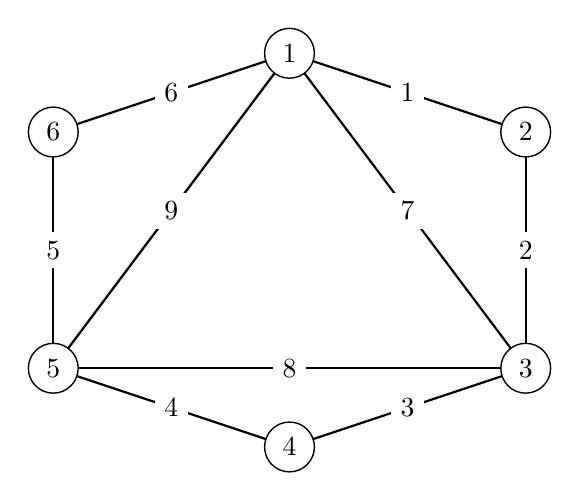
\begin{tikzpicture}
        \Vertex[x=0, y=0]{1}
        \Vertex[x=3, y=-1]{2}
        \Vertex[x=3, y=-4]{3}
        \Vertex[x=0, y=-5]{4}
        \Vertex[x=-3, y=-4]{5}
        \Vertex[x=-3, y=-1]{6}
        \Edge[label=$1$](1)(2)
        \Edge[label=$2$](2)(3)
        \Edge[label=$3$](3)(4)
        \Edge[label=$4$](4)(5)
        \Edge[label=$5$](5)(6)
        \Edge[label=$6$](6)(1)
        \Edge[label=$7$](1)(3)
        \Edge[label=$8$](3)(5)
        \Edge[label=$9$](5)(1)
    \end{tikzpicture}
\end{figure}

\noindent Zaprezentowany wyżej kontrprzykład obala stwierdzenie z zadania.
\end{document}